% ムック版 SF 考証記事：AMBAC は本当に効くのか（A4、2 段組）
% ビルド: report/mook/ で latexmk -lualatex mook.tex
% 図はすべて自作（TikZ／pgfplots とリポジトリのシミュレーション結果）。作品の画像は使用していない。
\documentclass[paper=a4paper,fontsize=10pt,twocolumn,column_gap=2zw,line_length=24zw,number_of_lines=46,head_space=18mm]{jlreq}
\usepackage{amsmath,amssymb}
\usepackage{graphicx,xcolor}
\usepackage{booktabs,array}
\usepackage{tikz,pgfplots}
\pgfplotsset{compat=1.18}
\usetikzlibrary{arrows.meta,positioning,decorations.markings,calc,shapes.geometric}
\usepackage[most]{tcolorbox}
\usepackage[hidelinks]{hyperref}
\usepackage{url}
\graphicspath{{./}{../../figures/}}
\newcommand{\repo}{https://github.com/okamasaya/simulation_AMBAC}
\setlength{\textfloatsep}{8pt plus 2pt minus 2pt}
\setlength{\floatsep}{6pt plus 2pt minus 2pt}
\setlength{\abovecaptionskip}{3pt}
\renewcommand{\arraystretch}{1.1}

\definecolor{accent}{HTML}{C8102E}
\definecolor{accent2}{HTML}{1F4E9A}
\definecolor{boxbg}{HTML}{F3F5F9}

% 見出しを雑誌風に
\newcounter{msec}
\makeatletter
\renewcommand{\section}{\@ifstar{\msecstar}{\msecbox}}
\newcommand{\msecstar}[1]{\par\addvspace{0.6\baselineskip}\noindent{\bfseries\color{accent2}#1}\par\nopagebreak\vspace{0.2\baselineskip}}
\makeatother
\newcommand{\msecbox}[1]{\par\addvspace{0.8\baselineskip}\refstepcounter{msec}%
  \noindent\colorbox{accent2}{\parbox{\dimexpr\linewidth-2\fboxsep}{\color{white}\bfseries\large\strut\themsec\quad #1}}%
  \par\nopagebreak\vspace{0.4\baselineskip}\nopagebreak}

% コラム枠
\newtcolorbox{column}[1]{enhanced,breakable,colback=boxbg,colframe=accent2,boxrule=0.6pt,arc=2pt,
  fonttitle=\bfseries\small,title={#1},left=4pt,right=4pt,top=3pt,bottom=3pt,fontupper=\small}
% 結論の枠
\newtcolorbox{verdict}{colback=white,colframe=accent,boxrule=1pt,arc=2pt,left=4pt,right=4pt,top=2pt,bottom=2pt,fontupper=\small\bfseries}

\begin{document}

\twocolumn[
\begin{@twocolumnfalse}
{\begin{tikzpicture}[remember picture,overlay]
\fill[accent2] ([yshift=-4mm]current page.north west) rectangle ([yshift=-1mm]current page.north east);
\fill[accent] ([yshift=-5.5mm]current page.north west) rectangle ([yshift=-4.6mm]current page.north east);
\end{tikzpicture}}
\vspace*{2mm}
{\small\color{accent}\bfseries SF考証の現在地 ― 宇宙世紀の物理を確かめる}\par\vspace{2mm}
{\fontsize{24pt}{30pt}\selectfont\bfseries AMBACは本当に効くのか}\par\vspace{2mm}
{\Large\bfseries 1981年のSF考証を、2026年のパソコンで検証する}\par\vspace{4mm}
\begin{minipage}{0.97\textwidth}
\noindent\rule{\textwidth}{0.4pt}\par\vspace{1mm}
\large
手足を振って宇宙で向きを変える。重い足を持って地上に立つ。関節にマグネットコーティングを施し、内部の骨格に動きを任せる――。
『機動戦士ガンダム』（1979年）とその続編を支えてきたSF設定は、放映から半世紀近く、多くのファンに真剣に考察されてきた。
本稿では、その中心にあるAMBAC（Active Mass Balance Auto Control）を、物理の式と物理エンジンを使って、手元のパソコンだけで試してみた。
結論を先に書くと、AMBACは物理的に成立する。そして、機体を速くしようとすると、次に問題になるのは「止め方」だった。
それは、作品世界の技術が歩んだ順番と、よく似ていた。\par\vspace{1mm}
\noindent\rule{\textwidth}{0.4pt}
\end{minipage}
\vspace{5mm}
\end{@twocolumnfalse}
]

\section{AMBACとは何か}

AMBACは、劇中の台詞ではなく、1981年のムック『ガンダムセンチュリー』\cite{gcentury}でSF考証として示されたとされる概念である。
宇宙空間では、押し返してくれる地面も空気もない。それでもモビルスーツが手足を振って向きを変えられるのはなぜか。
その答えが、「手足を動かした反作用で胴体を回す」というAMBACだった。

荒唐無稽に聞こえるかもしれないが、これは実際に起きる。
背中から落とされた猫が空中で体をひねって足から着地するのも、宇宙飛行士が何もつかまずに体の向きを変えられるのも、同じ原理である\cite{kane1969,kane1970}。
近年では、国際宇宙ステーションに滞在した宇宙飛行士が、脚を使った姿勢の制御をAMBACになぞらえて紹介し、ファンの間で話題になった。

ただし「成立する」ことと「劇中のように使える」ことは別の話だ。
本稿では、次の4つの問いを順に確かめていく。
\begin{enumerate}\setlength{\itemsep}{0pt}
\item AMBACで、本当に好きな向きに回れるのか。
\item 18メートルの巨体でも使えるのか。
\item 「足なんて飾り」は本当か。
\item 機体を速く動かすと、次に何が問題になるのか。
\end{enumerate}

\section{手足を振れば、本当に回れるのか}

\textbf{腕を振っても、戻せば元どおり}。
宇宙に浮かんだ人型のモデルで、腕を1本だけ前に振ると、胴体は反対向きに回る。
ところが、腕を元に戻すと胴体も元の向きに戻ってしまう。
外から力が働かない限り、体全体の「回る勢い」（角運動量）は0のままだからだ。
これでは、首を振っているのと変わらない。

\textbf{2本を「ずらして」回すと、少しずつ回る}。
そこで、腕と脚の2つの関節を、少しずらして動かす。腕を上げる→脚を上げる→腕を下ろす→脚を下ろす、というように、2つの関節の角度が「輪（ループ）」を描くように動かすのである（図\ref{fig:loop}）。
すると、元の姿勢に戻ったときに、胴体の向きだけが少しずれて残る。
人間大のモデルでは、1周あたり約3°だった。これを繰り返せば、どんな向きにでも回れる。

\begin{figure}[t]\centering
\begin{tikzpicture}[>=Stealth,scale=0.95]
% 関節空間
\draw[->] (0,0)--(3.6,0) node[below left,font=\scriptsize]{腕の角度};
\draw[->] (0,0)--(0,3.0) node[above right,font=\scriptsize,xshift=-2pt]{脚の角度};
\fill[accent!15] (1.8,1.4) ellipse (1.1 and 0.85);
\draw[accent,very thick,postaction={decorate},decoration={markings,mark=at position 0.12 with {\arrow{Stealth}},mark=at position 0.62 with {\arrow{Stealth}}}] (1.8,1.4) ellipse (1.1 and 0.85);
\node[font=\scriptsize,align=center] at (1.8,1.4) {囲んだ\\「面積」};
\node[font=\scriptsize,align=center,anchor=north] at (1.8,-0.25) {(a) 関節の動き：輪を描く};
% 胴体
\begin{scope}[xshift=5.0cm,yshift=1.3cm]
\draw[gray,thick,fill=gray!10] (-0.25,-0.7) rectangle (0.25,0.7);
\begin{scope}[rotate=-14]
\draw[accent2,very thick,fill=accent2!10] (-0.25,-0.7) rectangle (0.25,0.7);
\end{scope}
\draw[->,accent,thick] (0,1.05) arc (90:62:1.05);
\node[font=\scriptsize,align=center] at (0.15,-1.45) {(b) 1周ごとに\\胴体が少し回る};
\end{scope}
\end{tikzpicture}
\caption{AMBACの仕組み。2つの関節を輪を描くように動かすと、元の姿勢に戻っても胴体の向きだけがずれる。ずれの大きさは、輪が囲んだ「面積」（正確には、場所ごとの効きやすさを掛けて足し合わせたもの）で決まる。}\label{fig:loop}
\end{figure}

\textbf{回る角度は「速さ」ではなく「形」で決まる}。
面白いのは、1周でどれだけ回るかが、手足を動かす速さに関係なく、輪の形と大きさだけで決まることだ。
ゆっくり回しても、速く回しても、1周で回る角度は同じになる。
物理学では「幾何学的位相」と呼ばれ、落下する猫の問題として研究されてきた\cite{montgomery1993}。

\textbf{物理エンジンでも同じ答え}。
この計算を、ロボット研究で使われる物理エンジンMuJoCo\cite{todorov2012}でも確かめた。
腕1本の往復では$-16.04^\circ$、腕と脚の輪1周では約$+2.97^\circ$で、手で書いた計算と小数点以下まで一致した（図\ref{fig:snap}）。

\begin{figure}[t]\centering
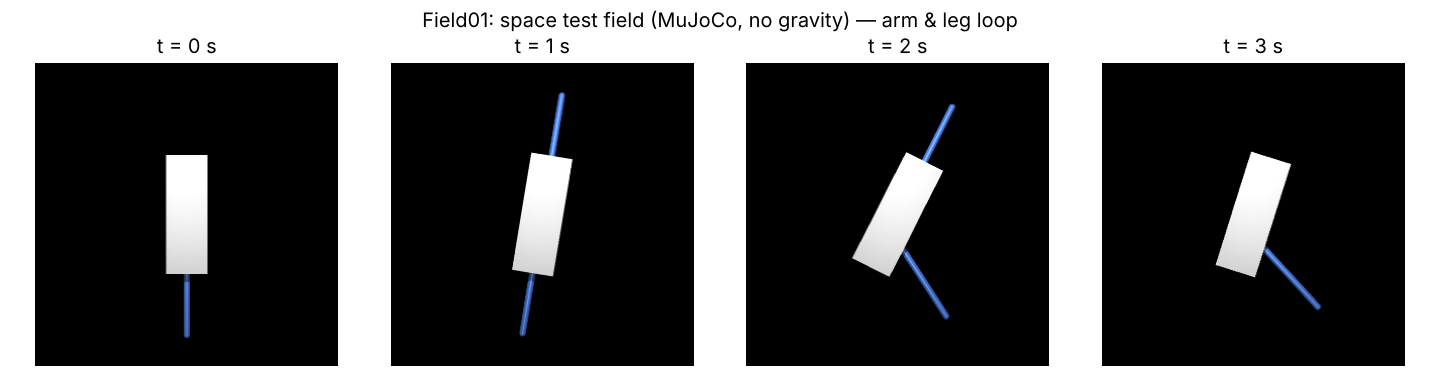
\includegraphics[width=\linewidth]{field/field01_snapshots.png}
\caption{物理エンジンの中の「宇宙の試験場」。白い胴体に腕と脚（青い棒）が付いた人型のモデルが、腕と脚で輪を描きながら向きを変えていく（0〜3秒）。}\label{fig:snap}
\end{figure}

\begin{verdict}
判定：AMBACは物理的に成立する。手足で輪を描けば、推進剤なしで好きな向きに回れる。
\end{verdict}

\begin{column}{コラム：人工衛星の「はずみ車」もAMBACの仲間}
人工衛星は、内部の円盤（リアクションホイール）を回して、その反作用で向きを変える。
これは、「どこまでも回し続けられる関節」を持ったAMBACだと考えると、同じ式で説明できる。
手足は可動域で止まってしまうので輪を描く必要があるが、円盤はぐるぐる回し続けられるので輪が要らない。
その代わり、円盤の回転には上限があり、上限に達すると推進剤で「勢いを捨てる」必要がある。
AMBACは、宇宙機の技術の延長線上にある。
\end{column}

\section{18メートルの壁}

では、全高18メートル級の機体でAMBACは使えるのか。
人間大のモデルをそのまま10倍に拡大（同じ密度で、重さは1000倍の約76トン）して計算した。

\textbf{回る角度は変わらない、でも遅くなる}。
輪1周で回る角度は、大きさによらず同じである。
問題は速さだ。長さが10倍になると、手足を同じ速さで振るのに必要な力（トルク）は10万倍（大きさの5乗）になる。
一方、同じ技術のモーターを相似に大きくしても、出せるトルクは1000倍（3乗）にしかならない。
いわゆる「二乗三乗則」である。

\begin{figure}[t]\centering
\begin{tikzpicture}
\begin{axis}[width=\linewidth,height=4.6cm,ybar,bar width=14pt,
  symbolic x coords={0.9 m,1.8 m,18 m,36 m},xtick=data,
  ylabel={90°の旋回 [秒]},ymin=0,ymax=310,
  nodes near coords,nodes near coords style={font=\scriptsize},
  every axis plot/.append style={fill=accent2!70,draw=accent2},
  xlabel={機体の大きさ（全高）},label style={font=\small},tick label style={font=\small},
  enlarge x limits=0.18]
\addplot coordinates {(0.9 m,6.6) (1.8 m,13) (18 m,132) (36 m,263)};
\end{axis}
\end{tikzpicture}
\caption{AMBACだけで90°向きを変えるのにかかる時間。モーターを相似に大きくした場合、時間は機体の大きさに比例して延びる。}\label{fig:scale}
\end{figure}

その結果、人間大なら十数秒で済む90°の旋回が、18メートル級では2分以上かかる（図\ref{fig:scale}）。
劇中のように数秒で機敏に向きを変えるには、相似に大きくしたモーターの約170倍、つまり\textbf{今のモーターより2桁以上強い「筋肉」}が必要になる。

逆に言えば、小さいほどAMBACは速い。猫が一瞬で体をひねれるのは、この法則の「小さい側」にいるからだ。

\textbf{スラスタとの役割分担}。
化学燃料のスラスタなら、90°を10秒で回るのに推進剤は約44kgで済む。
AMBACは推進剤を使わない代わりに遅い。
素早い旋回はスラスタに任せ、ゆっくりした向きの調整や、推進剤を節約したい場面ではAMBACを使う。
これが物理的に筋の通った使い方になる。
推進剤が尽きた、あるいは排気で位置を知られたくない、といった状況では、AMBACの「推進剤ゼロ」は決定的な利点になる。

\begin{verdict}
判定：巨大機でもAMBACは使えるが、遅い。劇中の機敏さには、2桁上の性能の関節が要る。
\end{verdict}

\section{「足なんて飾り」は本当か}

ファンなら誰でも知っている台詞がある。脚のない機体について、整備兵が「あんなの飾りです」と言う場面だ\cite{gundam}。
これが広まる過程で「足なんて飾りです」の形で知られるようになった。
では物理的に、脚は飾りなのか。答えは「場面による」だった（表\ref{tab:legs}）。

\textbf{宇宙では、脚は飾りではない}。
脚は腕より重く長いので、AMBACでは最も効く「重い手足」になる。
同じ総重量で比べると、脚を外した機体は、1周で稼げる回転が約4割減った（$9.6^\circ\to5.7^\circ$）。
逆に、推進剤タンクや装甲を脚に集めると、AMBACはさらに強くなる（$12.9^\circ$）。
皮肉なことに、台詞が語られた宇宙こそ、脚が最も役に立つ場面だった。
ただし、推進剤を惜しまずに使い切ってよい短時間の戦闘なら、スラスタだけで済むので、脚は飾りという判定にも理がある。

\textbf{地上の平地では、ほぼ飾り}。
二本脚で立つ機体は、足裏の支える範囲が狭く、重心が高い。
計算では、10kgの荷物を腕の先で持つだけで、止まっていても前に倒れた。
それでも人間が二本脚で荷物を持てるのは、\textbf{重い上体を後ろに反らせて釣り合いを取る}からだ。
上体を動かして腕の反作用を打ち消すこの動きは、いわば「地上版のAMBAC」である。
最適化の計算に任せると、人が重い物を持つときと同じ「反ってから前に傾く」動きを、自力で見つけ出した。
ただし、同じ上体を戦車型の台車に載せると、さらに速く、安定して運べた。

\textbf{段差では、人間大なら脚が強い}。
人間大の二本脚は、戦車型の2倍以上の段差を越えられる。
ところが、ここでも二乗三乗則が効く。18メートル級に拡大すると逆転し、相似に大きくしたモーターの脚では、わずか5cmの段差しか越えられなかった。

\begin{table}[t]\centering\small
\caption{「足は飾りか」の判定}\label{tab:legs}
\begin{tabular}{p{0.29\linewidth}p{0.17\linewidth}p{0.42\linewidth}}\toprule
場面 & 判定 & 理由 \\\midrule
宇宙 & \textbf{飾りではない} & 脚はAMBACで最も効く重い手足 \\
宇宙・短時間の戦闘 & 飾り & 推進剤を使い切ってよいならスラスタで足りる \\
地上・平地 & ほぼ飾り & 戦車型＋動く上体の方が速く安定 \\
地上・段差（人間大） & \textbf{飾りではない} & 戦車型の2倍以上の段差を越える \\
地上・段差（18m級） & 飾り & 二乗三乗則で5cmしか越えられない \\\bottomrule
\end{tabular}
\end{table}

\begin{verdict}
判定：「足は飾りか」は用途で決まる。だから、用途に合わせて下半身の形を選ぶ設計に意味がある。
\end{verdict}

\section{速くすると、次は「止め方」}

ここからは、現在進めている「第2段階」の話になる。
パソコンの中に「試験場」と「ステージ」を作り、部品表から機体を組み立てて動かす。
対戦ゲームの練習モードで、組み替えた機体を試すようなイメージだ。

試験の機体は、左右2本の履帯の台車に、10kgの荷物を持った腕を付けたもの。
腕を1秒で180°振ると、台車ごと約16°回ってしまった。
地上では、腕の反作用を足元の摩擦が受け止めてくれる。
ところが、反作用がある「境目」を超えると、その分だけ車体が回ったり滑ったりする。

\textbf{車体が回るのは、腕を「止めるとき」だった}。
詳しく調べると、腕を振り出すときの反作用は境目の内側に収まっていた。
境目を超えたのは、腕を\textbf{止めるとき}である。
腕を目標の位置に合わせる制御（位置サーボ）が遅れて腕が置いていかれ、最後に追いつこうとして急ブレーキになる。
その衝撃で、足元が滑っていた。
「何も考えずに速く動かすと、動きが雑に見える」原因の多くは、この「止め方」にあった。

対策を一つずつ試した結果は、直観に反するものもあった（表\ref{tab:stop}）。
関節にばねを入れて「しなり」を持たせると、かえって車体は大きく回った。
逆向きに回るおもりで反作用を打ち消すと向きは保てたが、速く振ると今度は横に倒れた。
最も安くて効いたのは、\textbf{止めるときの力を境目より下に抑えて、一定の力で止める}ことだった。
追加の部品なしで、車体をほとんど回さずに、むしろ速く振れた。

\begin{table}[t]\centering\small
\caption{腕を振ったときに車体が回る角度（荷物10kg、180°）}\label{tab:stop}
\begin{tabular}{lcc}\toprule
対策 & 振る時間 & 車体の回転 \\\midrule
なし（位置サーボ） & 1.0秒 & $+15.7^\circ$ \\
関節にしなり（ばね） & 1.0秒 & $+24.1^\circ$（悪化） \\
逆回転するおもり & 1.0秒 & $-1.4^\circ$ \\
逆回転するおもり & 0.6秒 & 横倒し \\
\textbf{止め方を変える} & \textbf{1.35秒} & $\mathbf{0.00^\circ}$ \\\bottomrule
\end{tabular}
\end{table}

\section{マグネットコーティングとムーバブルフレームを考え直す}

\textbf{「止める・保持する」専用の部品}。
止め方が鍵だと分かったので、次は「止める」ことを専門の部品に任せてみた。
使ったのは、MR流体（磁気粘性流体）のブレーキである。
MR流体は、細かい鉄の粒を油に混ぜた液体で、磁石の力をかけると一瞬で固くなり、磁力を弱めると元の液体に戻る。
つまり、\textbf{磁気で関節の「抵抗」を自在に変えられる}。
実際に、車のサスペンションや義足の膝などで使われている材料である。

モーターだけで「動かす・止める・保持する」をすべてこなす場合と、
「動かす＝モーター、止める・保持する＝MR流体」に分けた場合を比べた（図\ref{fig:split}、表\ref{tab:split}）。

\begin{figure}[t]\centering
\begin{tikzpicture}[font=\scriptsize,
  b/.style={draw,rounded corners=2pt,minimum height=0.62cm,align=center,text width=1.55cm},
  h/.style={font=\scriptsize\bfseries,align=center,text width=1.55cm}]
\node[h] at (0,0.2) {動かす};
\node[h] at (1.8,0.2) {止める};
\node[h] at (3.6,0.2) {保持する};
\node[anchor=east,font=\scriptsize] at (-1.0,-0.45) {モーターだけ};
\node[b,fill=gray!15,minimum width=5.15cm,text width=5.0cm] at (1.8,-0.45) {モーター（電力を使い続ける）};
\node[anchor=east,font=\scriptsize,align=right] at (-1.0,-1.25) {機能を分ける};
\node[b,fill=accent2!20] at (0,-1.25) {モーター};
\node[b,fill=accent!18,minimum width=3.35cm,text width=3.2cm] at (2.7,-1.25) {MR流体（磁気で制御）};
\node[anchor=east,font=\scriptsize] at (-1.0,-2.05) {人の体};
\node[b,fill=accent2!8] at (0,-2.05) {筋肉};
\node[b,fill=accent!8,minimum width=3.35cm,text width=3.2cm] at (2.7,-2.05) {靭帯・関節の摩擦};
\end{tikzpicture}
\caption{役割の分け方。動かす部品と、止める・保持する部品を分ける。人の体も、筋肉・腱・靭帯で役割を分けている。}\label{fig:split}
\end{figure}

\begin{table}[t]\centering\small
\caption{役割を分けた効果（荷物10kgの腕。段階15〜17の結果から）}\label{tab:split}
\setlength{\tabcolsep}{3pt}
\begin{tabular}{lcc}\toprule
 & モーターだけ & \textbf{モーター＋MR} \\\midrule
腕を180°振る時間 & 1.35秒 & \textbf{1.18秒} \\
目標からの行き過ぎ & 3.9° & \textbf{0.2°} \\
続けて動かせる頻度 & 毎分9.5回 & \textbf{毎分20.4回} \\
電源が落ちたとき & 腕が落ちて転倒 & \textbf{2mm下がるだけ} \\\bottomrule
\end{tabular}
\end{table}

結果は、速さ・正確さ・省エネ・安全が\textbf{同時に}よくなった。
止める仕事をMR流体に任せたことで、モーターは逆向きの力を出さずに済み、発熱がほぼ半分になった。
腕を上げたまま止まっているだけで、モーターは330Wの熱を出し続けるが、MR流体の保持なら電力は要らない。
そして、電源が落ちたとき、モーターだけの機体は腕が落ち、その勢いで車体まで倒れたが、MR流体は電源が切れた位置で腕をつかんだまま、2mmしか下がらなかった。

\textbf{作品世界の技術の順番}。
ここで、作品世界の技術を思い出してほしい。
初代では、主人公の機体の反応が、パイロットの操縦の速さについていけなくなり、関節にマグネットコーティングが施された。
設定では、磁気の力で関節の動きの遅れや抵抗を解消する技術とされる。
続編『機動戦士Ζガンダム』（1985年）\cite{zeta}では、内部の骨格（フレーム）が動きを受け持ち、装甲と役割を分ける「ムーバブルフレーム」が登場する。

本稿のシミュレーションがたどった順番は、これとよく似ている（図\ref{fig:timeline}）。
\begin{enumerate}\setlength{\itemsep}{0pt}
\item まず、手足を振って姿勢を変えられることを確かめた（AMBAC）。
\item 速く動かそうとすると、\textbf{関節の応答の遅れ}が急ブレーキを生み、機体を乱した。
\item その解決は、\textbf{磁気で関節の抵抗を制御する}部品（MR流体）だった。
\item さらに、\textbf{動かす部品と止める・保持する部品を分ける}と、すべての性能が同時によくなった。
\end{enumerate}
(2)(3)はマグネットコーティングに、(4)はムーバブルフレームの「役割を分ける」考え方に対応する。

\begin{figure}[t]\centering
\begin{tikzpicture}[font=\scriptsize,>=Stealth,
  s/.style={draw,rounded corners=2pt,align=center,text width=1.25cm,minimum height=0.95cm}]
\node[s,fill=gray!10] (a) at (0,0) {手足で\\向きを変える};
\node[s,fill=accent2!12] (b) at (1.75,0) {関節の\\応答の遅れ};
\node[s,fill=accent!15] (c) at (3.5,0) {磁気で\\関節を制御};
\node[s,fill=accent!28] (d) at (5.25,0) {動く部分と\\止める部分を分ける};
\draw[->,thick] (a)--(b); \draw[->,thick] (b)--(c); \draw[->,thick] (c)--(d);
\node[above=1pt of a,font=\scriptsize\bfseries] {作品世界};
\node[below=2pt of a,text width=1.5cm,align=center] {AMBAC\\（1981年の考証）};
\node[below=2pt of c,text width=1.6cm,align=center] {マグネット\\コーティング};
\node[below=2pt of d,text width=1.6cm,align=center] {ムーバブル\\フレーム（1985年）};
\node[below=2pt of b,text width=1.6cm,align=center] {反応が操縦に\\追いつかない};
\end{tikzpicture}
\vspace{2pt}
\begin{tikzpicture}[font=\scriptsize,>=Stealth,
  s/.style={draw,rounded corners=2pt,align=center,text width=1.25cm,minimum height=0.95cm}]
\node[s,fill=gray!10] (a) at (0,0) {Sim01〜05\\輪で回る};
\node[s,fill=accent2!12] (b) at (1.75,0) {段階13\\止めるときに\\車体が回る};
\node[s,fill=accent!15] (c) at (3.5,0) {段階14\\MR流体で\\止める};
\node[s,fill=accent!28] (d) at (5.25,0) {段階15〜17\\モーターと\\MRを分ける};
\draw[->,thick] (a)--(b); \draw[->,thick] (b)--(c); \draw[->,thick] (c)--(d);
\node[above=1pt of a,font=\scriptsize\bfseries] {本稿のシミュレーション};
\end{tikzpicture}
\caption{作品世界の技術の順番（上）と、本稿のシミュレーションがたどった順番（下）。}\label{fig:timeline}
\end{figure}

もちろん、違いもある。
設定のマグネットコーティングは、関節の抵抗を\textbf{減らして}速くする技術であり、MR流体は、抵抗を\textbf{増やして}止める・保持する技術だ。
向きは逆だが、共通しているのは、\textbf{関節の抵抗を、場面ごとに磁気で制御する}という発想である。
速く動かしたいときは抵抗を消し、止めたいときは抵抗を足す。
今回の結果は、その両方が要ることを示している。

1979年から1985年当時に知られていた基礎――角運動量の保存、関節の応答、材料の性質――の上に立って、
「機体を速くすると、次は関節の性質と止め方が問題になり、その次は役割を分けた構造が要る」と考えたのだとすれば、
それは、私たちのシミュレーションが示した最適解に近い方向を、先に指していたことになる。
設定がどこまで意図したものかは分からない。
ただ、\textbf{当時の基礎理論から考え抜かれたSF考証は、検証できる仮説として今も通用する}、とは言えそうだ。

\begin{verdict}
考察：マグネットコーティングとムーバブルフレームは、「関節の抵抗を磁気で制御する」「動く部分と止める部分を分ける」という、物理的に筋の通った解決策と読める。
\end{verdict}

\begin{column}{コラム：AIはAMBACを自力で発見できるか}
「胴体を目標の向きまで回せ」とだけ教えて、AIに手足の動かし方を学ばせてみた。
物理の知識を何も与えないと、AIは手足を可動域の端まで振り切って止まる、という間違った答えにはまり込んだ。
輪の効果は、振る幅の2乗でしか効かないため、小さな動きから学び始めると「輪を大きくすればよい」という手がかりがほとんど得られないのだ。
ところが、「輪を描く」という\textbf{形}だけを与えると、AIは人間が設計した円い輪より効率のよい輪を見つけ、理論上の上限の98\%に達した。
物理の「形」は人間が与え、細かい調整はAIに任せる。これは、今のロボット開発でも重要な考え方である。
\end{column}

\section{舞台裏：実機もGPUもない}

ここで、正直に書いておかなければならないことがある。
この検証には、\textbf{実物のロボットが1台もない}。
そして、映像のように精細なシミュレーションや、大規模なAIの学習には最新世代のGPUが必要とされるが、それも手元にはない。
すべての計算は、普通のパソコンのCPUだけで行った。

そのため、本稿の数値には限界がある。
\begin{itemize}\setlength{\itemsep}{0pt}
\item モーターやMR流体の数値は、仮定した部品の値である。実在の製品に当てはめるには、カタログの値に置き換える必要がある。
\item 部品のたわみ、接触の細かい様子、流体の温度むらなど、モデルに入れていない現象は再現されない。
\item シミュレーションと現実のずれ（いわゆるsim-to-realの問題）そのものは、パソコンの上だけでは確かめられない。
\end{itemize}

それでも、安いシミュレーションにできることはあった。
まず、\textbf{答えの分かっている問題で、シミュレーター自体を試験する}ことだ。
手で書いた式と物理エンジンを照合し、小数点以下まで一致することを確かめてから先に進んだ。
次に、\textbf{答えを隠した「仮想の実機」}を作った。
重さや慣性をこっそりずらした機体を用意し、手足の輪の動きと胴体の揺れだけから、隠した値を誤差約2\%で当てられることを確かめた。
実機が手に入ったときに、何をどう測ればよいかを、先に決めておけるわけだ。
そして、動画で目で確かめることで、床を突き抜けた腕や、電源を切った後にゆっくり落ちる腕など、数値だけでは見落とす不具合をいくつも見つけた。

安いシミュレーションは、実機の代わりにはならない。
しかし、\textbf{実機に何を持ち込むべきかを決める道具}にはなる。
次の目標は、安価なサーボで組んだ腕1本を「3層目」として、式・シミュレーション・実機の3つを照合することである。

\section{おわりに}

AMBACは物理的に成立する。ただし巨大機では遅く、脚が飾りかどうかは用途で決まる。
そして、機体を速くしようとすると、問題は「止め方」に移り、その答えは「関節の抵抗を磁気で制御し、動く部分と止める部分を分ける」ことだった。
半世紀近く前のSF設定と、2026年のパソコンの計算が、同じ順番をたどったことは偶然かもしれない。
それでも、ファンが真剣に考察してきたSF設定は、検証できる仮説の宝庫である。
本稿の計算はすべて公開しているので、ぜひ自分の手で、あの機体を動かしてみてほしい\footnote{\url{\repo}}。

\vspace{2mm}
\begin{thebibliography}{9}\footnotesize\setlength{\itemsep}{0pt}
\bibitem{gundam} 『機動戦士ガンダム』（テレビアニメ, 1979年, 日本サンライズ）. 第42話「宇宙要塞ア・バオア・クー」.
\bibitem{gcentury} 『ガンダムセンチュリー』（みのり書房, 1981年）. 復刻版：『GUNDAM CENTURY RENEWAL VERSION 宇宙翔ける戦士達』（樹想社, 2000年）.
\bibitem{zeta} 『機動戦士Ζガンダム』（テレビアニメ, 1985年, 日本サンライズ）.
\bibitem{kane1969} T.~R.~Kane, M.~P.~Scher, ``A dynamical explanation of the falling cat phenomenon,'' \textit{Int. J. Solids and Structures}, 5(7), 1969.
\bibitem{kane1970} T.~R.~Kane, M.~P.~Scher, ``Human self-rotation by means of limb movements,'' \textit{J. Biomechanics}, 3(1), 1970.
\bibitem{montgomery1993} R.~Montgomery, ``Gauge theory of the falling cat,'' Fields Inst. Commun. 1, AMS, 1993.
\bibitem{todorov2012} E.~Todorov, T.~Erez, Y.~Tassa, ``MuJoCo: A physics engine for model-based control,'' \textit{IROS}, 2012.
\end{thebibliography}
{\scriptsize 本稿の図は、すべて筆者のシミュレーション結果と自作の図解である。作品名・設定名は考察のために引用した。}

\end{document}
